\documentclass[a4paper]{article}
\usepackage[utf8]{inputenc}
\usepackage[russian,english]{babel}
\usepackage[T2A]{fontenc}
\usepackage[left=10mm, top=20mm, right=18mm, bottom=15mm, footskip=10mm]{geometry}
\usepackage{indentfirst}
\usepackage{amsmath,amssymb}
\usepackage{mathastext} 
\usepackage[italicdiff]{physics}
\usepackage{graphicx}
\usepackage{caption}
\usepackage{float}
\usepackage{caption}
\renewcommand{\thefootnote}{\fnsymbol{footnote}}
\usepackage{tablefootnote}
\usepackage{footmisc}
\usepackage{textcomp}
\usepackage{multicol}
\usepackage{multirow}
\usepackage[parfill]{parskip}
\usepackage{makecell}
\usepackage{array}  
\usepackage{siunitx}
\usepackage{booktabs}
\sisetup{
    exponent-product = \cdot,
    per-mode = symbol,
    separate-uncertainty = true,
    uncertainty-separator = \,
}
\renewcommand\cellalign{cc} 
\renewcommand\cellgape{\Gape[2pt]} 
\usepackage[utf8]{inputenc}\newcommand{\approxtext}[1]{\ensuremath{\stackrel{\text{#1}}{\approx}}}
\usepackage[colorlinks=true, urlcolor=blue, linkcolor=blue, citecolor=blue]{hyperref}
\graphicspath{{images/}}
\DeclareGraphicsExtensions{.pdf,.png,.jpg}
\usepackage{wrapfig}
\captionsetup{labelformat=empty}
\usepackage{caption}
\captionsetup[figure]{name=Рисунок}
\captionsetup[table]{name=Таблица}
%\usepackage{newtxtext,newtxmath} 
\title{\textbf{Отчет о выполнении лабораторной работы 4.3.2} \\[0.5em] \large\itshape Дифракция света на ультразвуковой волне в жидкости}
\date{}
\author{Котляров Михаил, Б01-402}

\begin{document}

\maketitle
	
\section{Введение}

\subsubsection*{Цель работы:} Изучение дифракции света на синусоидальной акустической решётке и наблюдение фазовой решётки методом тёмного поля.

\subsubsection*{Оборудование и инструментальные погрешности}

\textbf{оптическая скамья},\\
\textbf{осветитель},\\
\textbf{два длиннофокусных объектива}: фокусное расстояние $f = 30$ см,\\
\textbf{кювета с жидкостью},\\
\textbf{генератор ультразвуковой частоты Г3-112}: погрешность частоты в диапазоне 1 МГц – 10 МГц составляет $\pm 3$ \%,\\
\textbf{кварцевый излучатель с микрометрическим винтом},\\
\textbf{линза}: фокусное расстояние $f = 110$ см,\\
\textbf{вертикальная нить на рейтере},\\
\textbf{микроскоп}: точность и цена деления неизвестны. Шкала не использовалась для прямых измерений,\\
\textbf{Частотомер GW instek GFC-8010H}: погрешность измерения определялась по последнему разряду \textbf{записанной частоты}, поскольку частотомер измеряет намного точнее.

\subsection{Описание экспериментальной установки}

Экспериментальная установка для наблюдения дифракции света на ультразвуковых волнах в жидкости представлена на рис.~\ref{fig:scheme}. Оптическая схема собрана на оптической скамье и включает следующие основные элементы:

\begin{itemize}
    \item \textbf{Источник света~$\mathbf{Л}$} --- обеспечивает освещение щели;
    \item \textbf{Светофильтр~$\mathbf{\Phi}$} --- монохроматизирует излучение (в работе используется красный светофильтр);
    \item \textbf{Конденсор~$\mathbf{К}$} --- формирует равномерное освещение щели;
    \item \textbf{Щель~$\mathbf{S}$} --- расположена в фокальной плоскости объектива~$O_1$, служит источником когерентного света;
    \item \textbf{Объектив~$\mathbf{O_1}$} --- коллимирует свет, формируя параллельный пучок ($f = 30$~см);
    \item \textbf{Кювета~$\mathbf{C}$} --- содержит воду, в которой распространяется ультразвуковая волна;
    \item \textbf{Пьезокварцевый излучатель~$\mathbf{Q}$} --- закреплён на стенке кюветы, возбуждает УЗ-волны при подаче синусоидального напряжения от генератора;
    \item \textbf{Микрометрический винт} --- позволяет перемещать излучатель для точной настройки стоячей волны, цена деления винта 4 мкм;
    \item \textbf{Объектив~$\mathbf{O_2}$} --- фокусирует прошедший через кювету свет в своей фокальной плоскости~$F$ ($f = 30$~см);
    \item \textbf{Отсчётное устройство} --- содержит микрометрический винт~$B$, реперную линию~$л$, перекрестье~$П$ и проволоку~$П_{\text{р}}$ для метода тёмного поля;
    \item \textbf{Микроскоп~$\mathbf{M}$} --- для наблюдения дифракционной картины в фокальной плоскости~$F$;
    \item \textbf{Генератор ультразвуковой частоты и частотомер} --- для задания и контроля частоты~$\nu$ колебаний излучателя.
\end{itemize}

\begin{figure}[h!]
\centering
  
\includegraphics[width=0.8\linewidth]{Pictures/setup.png}
  \caption{Рис. 1. Схема установки}
\label{fig:scheme}
\end{figure}

\begin{figure}[h!]
\centering
  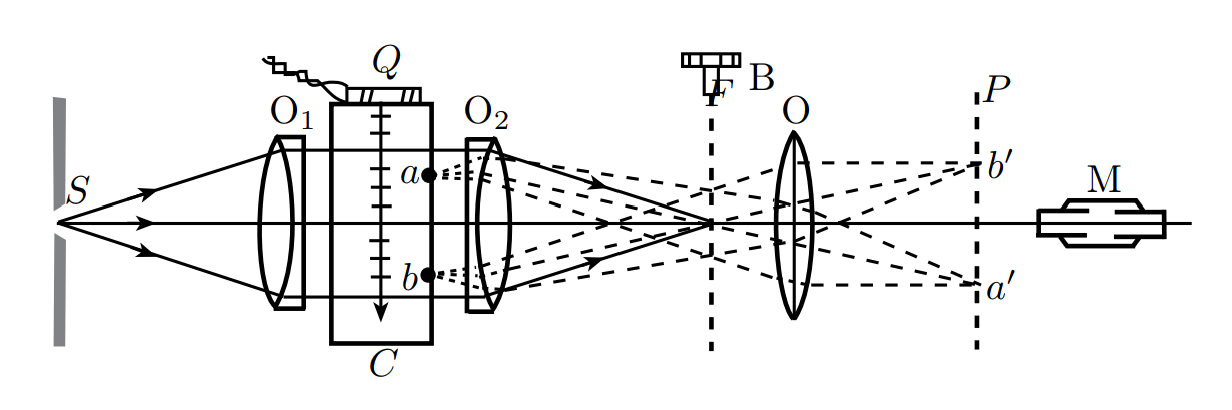
\includegraphics[width=0.8\linewidth]{Pictures/setup-2.png}
  \caption{Рис. 2. Схема установки для измерения методом тёмного поля}
\label{fig:scheme2}
\end{figure}

\subsubsection*{Принцип работы установки}

Свет от источника~$Л$, пройдя через светофильтр~$\Phi$ и конденсор~$К$, освещает щель~$S$. Щель расположена в фокусе объектива~$O_1$, поэтому выходящий из него пучок является параллельным. Этот пучок проходит через кювету~$C$ перпендикулярно направлению распространения ультразвуковой волны, возбуждаемой пьезокварцевой пластинкой~$Q$.

В результате взаимодействия света с периодической структурой показателя преломления, создаваемой УЗ-волной, в фокальной плоскости~$F$ объектива~$O_2$ формируется дифракционная картина --- система вертикальных полос (максимумов порядков $m = 0, \pm 1, \pm 2, \ldots$). Картина наблюдается через микроскоп~$M$.

Координаты максимумов $x_m$ измеряются с помощью микрометрического винта отсчётного устройства по положению перекрестья~$П$. Для повышения точности измерений используется монохроматический свет (красный светофильтр), а все измерительные элементы (линия~$л$, перекрестье~$П$, проволока~$П_{\text{р}}$) расположены в плоскости резкого изображения щели~$F$.

\subsection{Метод тёмного поля}

Для наблюдения изображения самой акустической решётки применяется метод тёмного поля. \\В этом случае (см ~\ref{fig:scheme2}):
\begin{enumerate}
    \item За отсчётным устройством устанавливается дополнительная линза~$O$;
    \item Микроскоп перемещается вдоль скамьи и фокусируется на изображение задней стенки кюветы;
    \item Проволока~$П_{\text{р}}$ вводится в оптический путь для перекрытия центрального (нулевого) дифракционного максимума;
    \item В поле зрения микроскопа наблюдаются чередующиеся светлые и тёмные полосы, расстояние между которыми соответствует $\Lambda/2$, где $\Lambda$ --- длина УЗ-волны.
\end{enumerate}

Важно: метод тёмного поля применим только для стоячих ультразвуковых волн, так как в случае бегущей волны визуальное наблюдение структуры невозможно из-за высокой частоты колебаний.

\section{Ход работы и результаты измерений}

\subsection{Определение скорости ультразвука по дифракционной картине}

\begin{enumerate}

\item \textbf{Настройка оптической схемы.} Соберём оптическую схему согласно рис.~\ref{fig:scheme}. Щель~$S$ установим на фокусном расстоянии от объектива~$O_1$ ($f = 30$~см). Ярко осветим щель с помощью конденсора~$К$, предварительно используя зелёный светофильтр. Убедимся, что световое пятно на щели равномерно освещено. Затем с помощью листа бумаги найдём резкое изображение щели~$S$ в фокальной плоскости~$F$ объектива~$O_2$. В случае необходимости отцентрируем источник света и конденсор. Настроим микроскоп~$M$ и отсчётное устройство.

\item \textbf{Получение дифракционной картины.} Включим генератор ультразвуковой частоты и получим в поле зрения микроскопа систему дифракционных полос. Картина наблюдается наиболее чётко при образовании в кювете стоячей УЗ-волны. Заменим широкополосный зелёный фильтр на красный монохроматический. Изменяя ширину щели~$S$, её наклон и положение конденсора, добьёмся оптимальных условий наблюдения дифракционных полос.

\item \textbf{Измерения координат максимумов.} Для 5 частот $\nu$определим положения $x_m$ шести--восьми дифракционных максимумов ($m = 1, 2, \ldots, N$) с помощью микрометрического винта отсчётного устройства по перекрестью. Погрешность $x_m$ оценена в 20 мкм, поскольку при повторном измерении одного и того же максимума значение изменялось на $\pm$ 5 делений микрометрического винта.

% === Первая строка: три таблицы ===
\begin{table}[h!]
    \centering
    \begin{minipage}[t]{0.3\textwidth}
        \centering
        \begin{tabular}{|c|c|}
            \hline
            $m$ & $x_m$, мкм \\ \hline
            1 & 152 \\ \hline
            2 & 304 \\ \hline
            3 & 436 \\ \hline
            4 & 584 \\ \hline
            5 & 708 \\ \hline
            6 & 844 \\ \hline
            7 & 976 \\ \hline
            8 & 1096 \\ \hline
        \end{tabular}
        \caption{Таблица 1. \\$\nu = 1{,}02$ МГц}
        \label{tab:freq1}
    \end{minipage}%
    \hfill
    \begin{minipage}[t]{0.3\textwidth}
        \centering
        \begin{tabular}{|c|c|}
            \hline
            $m$ & $x_m$, мкм \\ \hline
            1 & 136 \\ \hline
            2 & 272 \\ \hline
            3 & 404 \\ \hline
            4 & 556 \\ \hline
            5 & 704 \\ \hline
            6 & 844 \\ \hline
            7 & 996 \\ \hline
            8 & 1132 \\ \hline
        \end{tabular}
        \caption{Таблица 2. \\$\nu = 1{,}095$ МГц}
        \label{tab:freq2}
    \end{minipage}%
    \hfill
    \begin{minipage}[t]{0.3\textwidth}
        \centering
        \begin{tabular}{|c|c|}
            \hline
            $m$ & $x_m$, мкм \\ \hline
            1 & 80 \\ \hline
            2 & 160 \\ \hline
            3 & 316 \\ \hline
            4 & 472 \\ \hline
            5 & 636 \\ \hline
            6 & 788 \\ \hline
            7 & 952 \\ \hline
        \end{tabular}
        \caption{Таблица 3. \\$\nu = 1{,}20$ МГц}
        \label{tab:freq3}
    \end{minipage}
\end{table}

% === Вторая строка: две таблицы ===
\begin{table}[h!]
    \centering
    \begin{minipage}[t]{0.5\textwidth}
        \centering
        \begin{tabular}{|c|c|}
            \hline
            $m$ & $x_m$, мкм \\ \hline
            1 & 160 \\ \hline
            2 & 320 \\ \hline
            3 & 488 \\ \hline
            4 & 660 \\ \hline
            5 & 808 \\ \hline
            6 & 980 \\ \hline
            7 & 1136 \\ \hline
        \end{tabular}
        \caption{Таблица 4. \\$\nu = 1{,}27$ МГц}
        \label{tab:freq4}
    \end{minipage}%
    \hfill
    \begin{minipage}[t]{0.5\textwidth}
        \centering
        \begin{tabular}{|c|c|}
            \hline
            $m$ & $x_m$, мкм \\ \hline
            1 & 176 \\ \hline
            2 & 352 \\ \hline
            3 & 536 \\ \hline
        \end{tabular}
        \caption{Таблица 5. \\ $\nu = 1{,}36$ МГц}
        \label{tab:freq5}
    \end{minipage}
\end{table}

\item \textbf{Построение графиков и определение наклона.} Для каждой частоты По взвешенному методу наименьших квадратов построим график зависимости координаты максимума $x_m$ от его порядка $m$.

\clearpage
\begin{figure}[h!]
\centering
  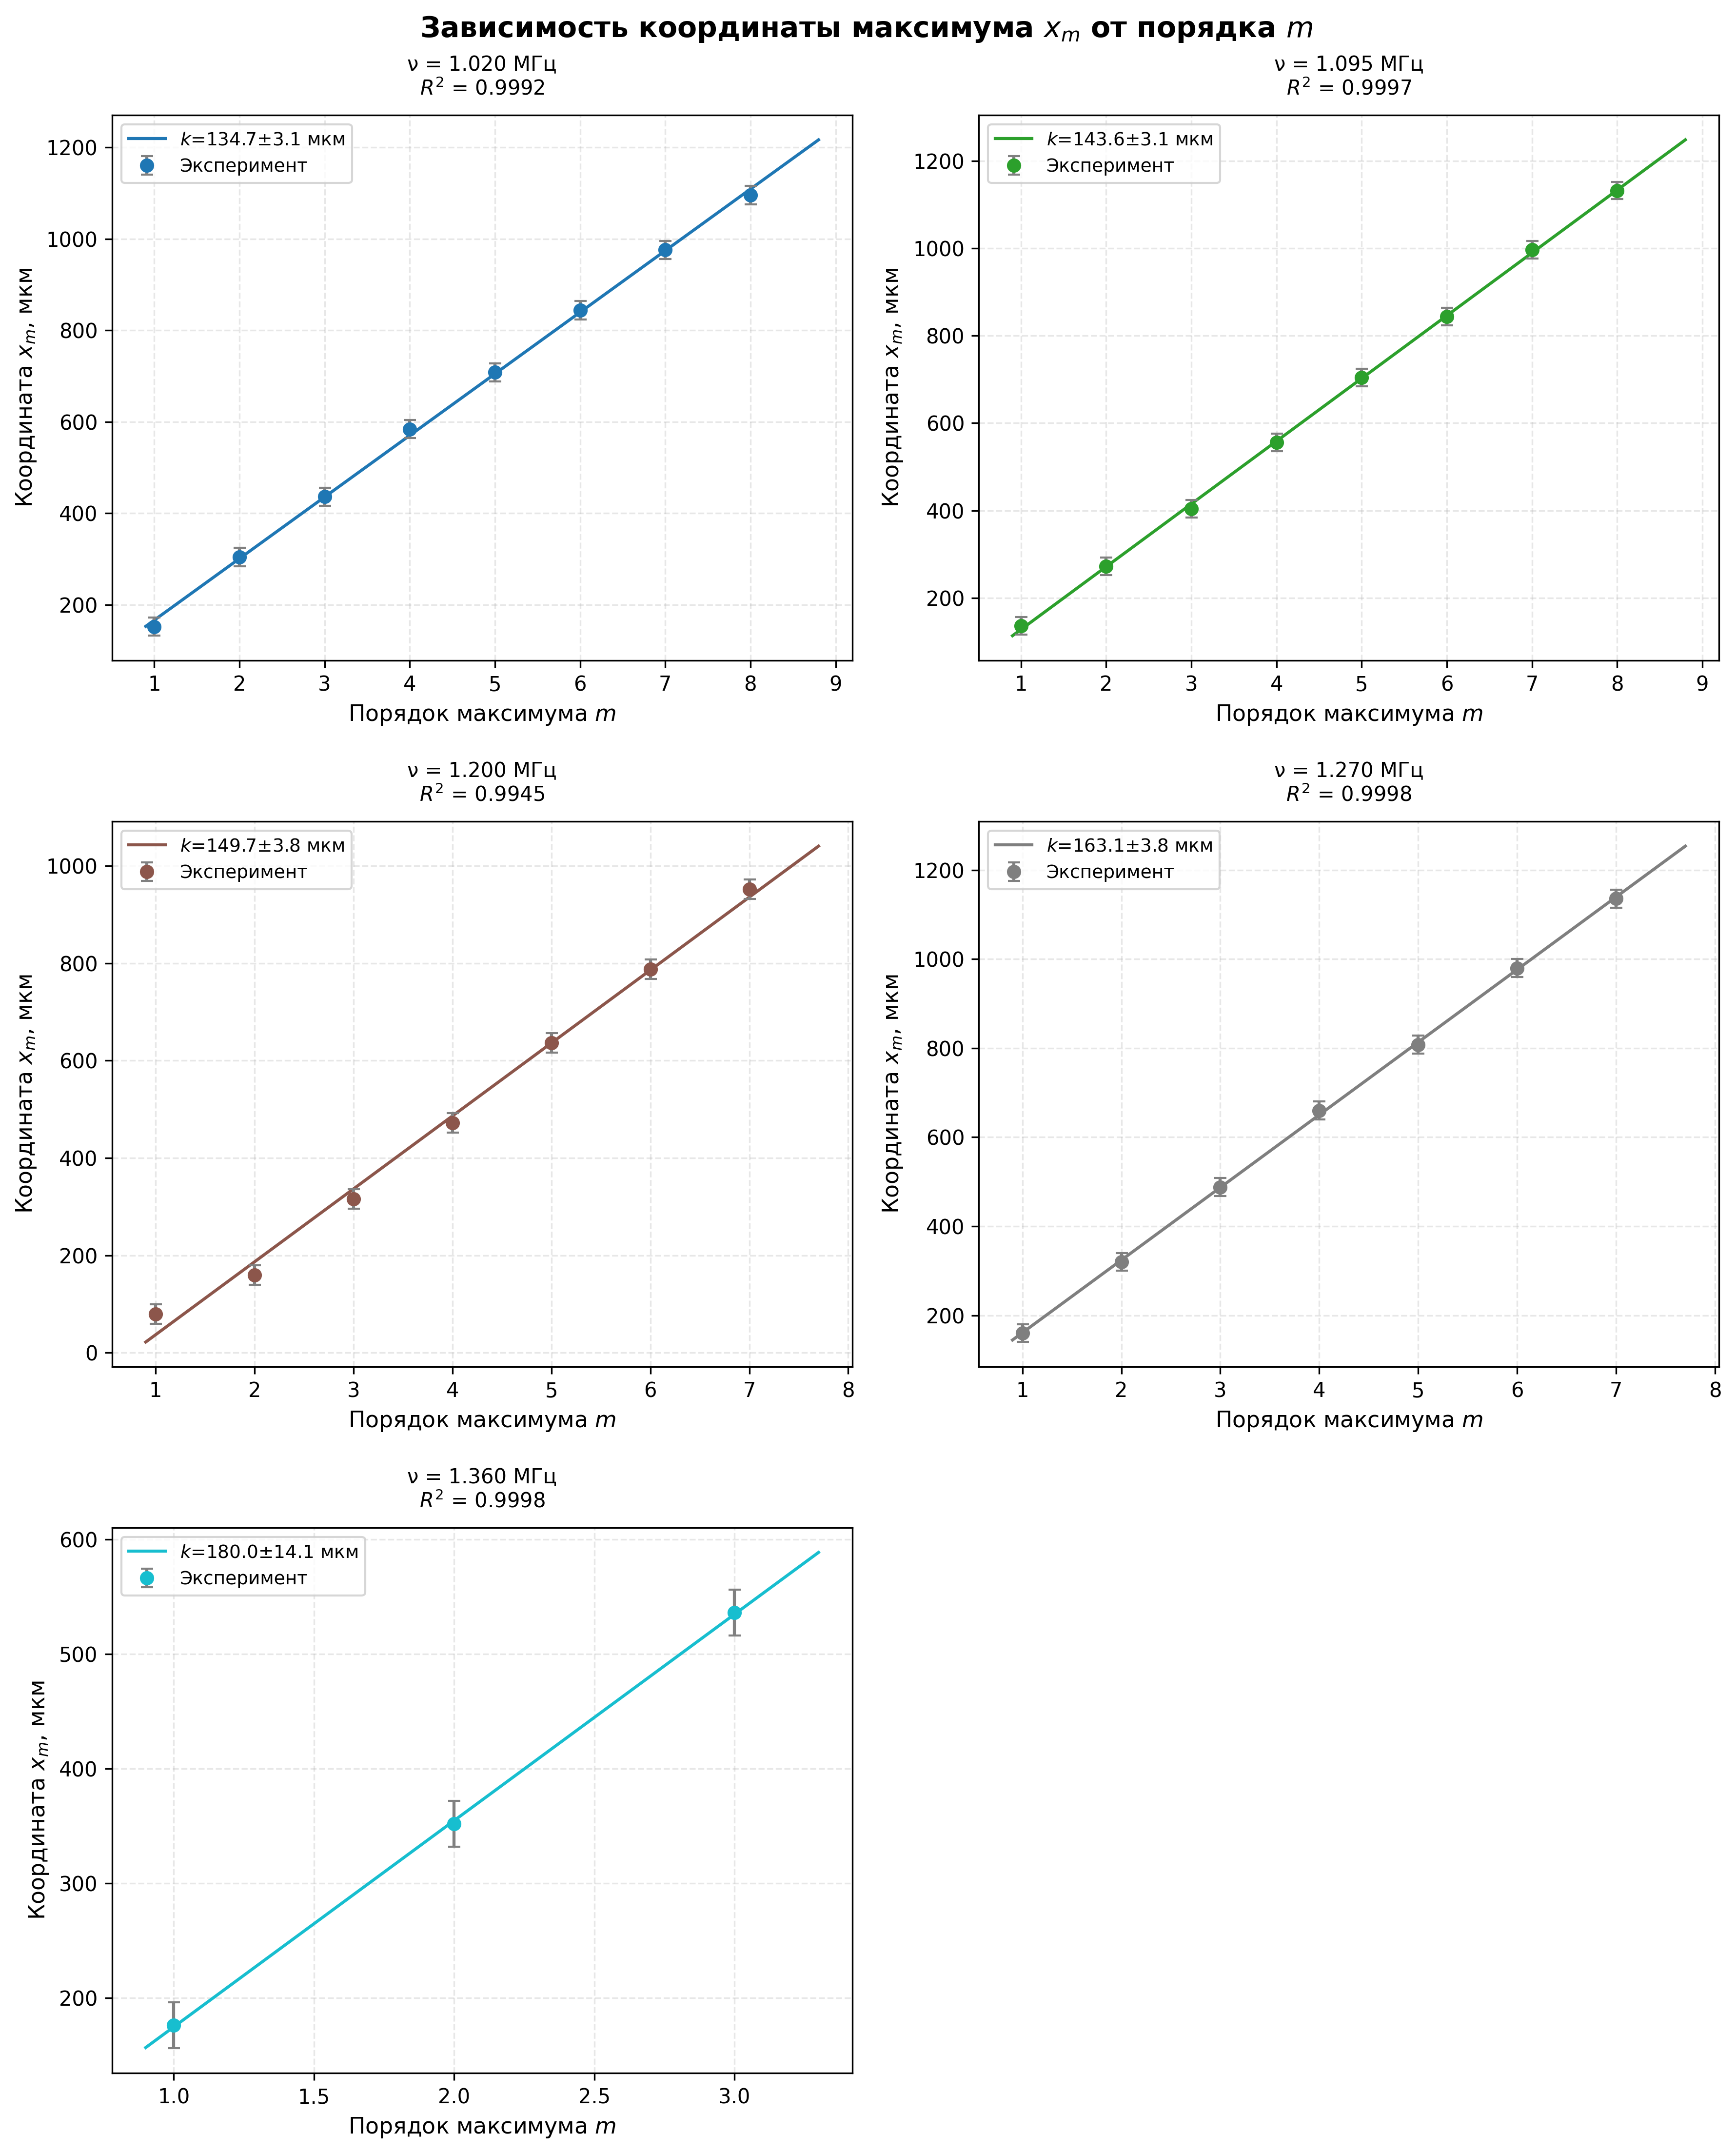
\includegraphics[width=1\linewidth]{Graphics/diffraction_plots.png}
  \caption{График 1. Зависимости координаты максимума $x_m$ от его порядка $m$}
\end{figure}

\item \textbf{Расчёт длины УЗ-волны и скорости звука.} Для каждой частоты рассчитаем длину УЗ-волны:
$$
\Lambda = \frac{f \lambda}{k}.
$$
Затем по формуле~(5) определим скорость ультразвука:
$$
v = \Lambda \nu.
$$

Результаты сведем в таблицу.

\begin{table}[h!]
\centering

\begin{tabular}{|c|c|c|c|c|c|c|}
\hline
$\nu$, МГц & 
$k$, мкм & 
$\varepsilon_k$, \% & 
$\Lambda$, мм & 
$\varepsilon_\Lambda$, \% & 
$v$, м/с & 
$\varepsilon_v$, \% \\
\hline
1,020 & $134{,}71 \pm 3{,}09$ & 2,29 & 
$1{,}425 \pm 0{,}055$ & 3,88 & 
$1454 \pm 71$ & 4,90 \\ \hline
1,095 & $143{,}57 \pm 3{,}09$ & 2,15 & 
$1{,}337 \pm 0{,}051$ & 3,79 & 
$1464 \pm 71$ & 4,84 \\ \hline
1,200 & $149{,}71 \pm 3{,}78$ & 2,52 & 
$1{,}282 \pm 0{,}052$ & 4,02 & 
$1539 \pm 77$ & 5,01 \\ \hline
1,270 & $163{,}14 \pm 3{,}78$ & 2,32 & 
$1{,}177 \pm 0{,}046$ & 3,89 & 
$1495 \pm 73$ & 4,91 \\ \hline
1,360 & $180 \pm 14$ & 7,86 & 
$1{,}067 \pm 0{,}090$ & 8,45 & 
$1451 \pm 130$ & 8,97 \\ \hline
\end{tabular}%

\caption{Таблица 6. Результаты измерений и расчётов скорости ультразвука}
\label{tab:results}
\end{table}

\item \textbf {Обработка результатов и нахождение средней скорости звука}

\textbf {Методика усреднения.} Поскольку измерения скорости звука проводились на пяти различных частотах и для каждого значения $v_i$ была определена полная погрешность, для нахождения наилучшей оценки истинного значения скорости звука использовали метод взвешенного среднего с разделением случайных и систематических погрешностей.

\textbf {Разделение погрешностей.} Для каждого измерения $v_i$ полная погрешность $\sigma_i$ была представлена как квадратичная сумма:
\begin{equation}
    \sigma_i^2 = \sigma_{i,\text{сл}}^2 + \sigma_{\text{сист}}^2,
\end{equation}
где:
\begin{itemize}
    \item $\sigma_{i,\text{сл}} = v_i \cdot \dfrac{\sigma_k^{(i)}}{k_i}$ --- случайная погрешность, обусловленная неопределённостью наклона графика $x_m(m)$ (различна для каждой частоты);
    \item $\sigma_{\text{сист}}$ --- систематическая погрешность, одинаковая для всех измерений и обусловленная неточностью известных параметров установки: фокусного расстояния $f$ и длины волны света $\lambda$.
\end{itemize}

Систематическая погрешность оценивалась по формуле:
\begin{equation}
    \sigma_{\text{сист}} = \langle v \rangle_{\text{w}} \cdot 
    \sqrt{  \varepsilon_\nu ^2 + \left( \frac{\Delta \lambda}{\lambda} \right)^2 },
\end{equation}
где $\varepsilon_\nu = 0,03 \ (3\%)$, $\Delta \lambda = 20$~нм, $\lambda = 640$~нм (красный свет) --- погрешности параметров, указанные в технической документации.

\textbf {Взвешенное среднее.} Веса для усреднения определялись только случайными погрешностями:
\begin{equation}
    w_i = \frac{1}{\sigma_{i,\text{сл}}^2}.
\end{equation}

Взвешенное среднее значение скорости звука:
\begin{equation}
    \langle v \rangle_w = \frac{\sum\limits_{i=1}^{N} w_i v_i}{\sum\limits_{i=1}^{N} w_i}.
\end{equation}

\textbf {Погрешность среднего.} Случайная составляющая погрешности среднего:
\begin{equation}
    \sigma_{\text{средн,сл}} = \sqrt{ \frac{1}{\sum\limits_{i=1}^{N} w_i} }.
\end{equation}

Систематическая составляющая не уменьшается при усреднении, так как является коррелированной для всех измерений:
\begin{equation}
    \sigma_{\text{средн,сист}} = \sigma_{\text{сист}}.
\end{equation}

Полная погрешность результата находится как квадратичная сумма:
\begin{equation}
    \sigma_{\text{полн}} = \sqrt{ \sigma_{\text{средн,сл}}^2 + \sigma_{\text{средн,сист}}^2 }.
\end{equation}

\textbf {Результаты расчётов.} На основе данных таблицы~\ref{tab:results} были получены следующие значения:

\begin{table}[h!]
\centering

\begin{tabular}{|l|c|}
\hline
Параметр & Значение \\
\hline
Систематическая погрешность среднего, $\sigma_{\text{ср}}^{\text{сист}}$, м/с & $64{,}23$ \\ \hline
Взвешенное среднее, $\langle v \rangle_w$, м/с & $1482{,}80$ \\ \hline
Случайная погрешность среднего, $\sigma_{\text{средн,сл}}$, м/с & $16{,}95$ \\ \hline
Полная погрешность, $\sigma_{\text{полн}}$, м/с & $66{,}43$ \\ \hline
Относительная погрешность, $\varepsilon$, \% & $4{,}48$ \\ \hline
\end{tabular}
\caption{Таблица 7. Параметры взвешенного усреднения скорости звука}
\label{tab:weighted_avg}
\end{table}

\textbf {Итоговый результат.} Окончательное значение скорости ультразвука в воде при температуре эксперимента:
\begin{equation}
    \boxed{ v = (1483 \pm 66)~\text{м/с}, \quad \varepsilon = 4{,}5\% }.
\end{equation}

\textbf {Сравнение с теорией.}
 Теоретическое значение скорости звука в воде при $20^\circ$C составляет $v_{\text{теор}} \approx 1481$\footnotemark[1] ~м/с. Полученный результат:
\begin{itemize}
    \item Отклонение от теории: $\Delta = |1483 - 1481| = 2$~м/с ($0{,}2\%$);
    \item Отклонение находится в пределах экспериментальной погрешности ($2 < 66$~м/с).
\end{itemize}
Таким образом, экспериментальные данные согласуются с теоретическими предсказаниями в пределах точности измерений.
\footnotetext[1]{Значение взято для воды при 20$^\circ$ \url{https://dpva.ru/Guide/GuideMedias/GuideWater/TemperatureSoundSpeed/}, время обращения 1.03.2026}

\textbf {Анализ вклада погрешностей.} Из таблицы~\ref{tab:weighted_avg} видно, что доминирующий вклад в полную погрешность вносит систематическая составляющая ($\sigma_{\text{сист}} \approx 64$~м/с против $\sigma_{\text{сл}} \approx 17$~м/с). Это связано с тем, что погрешность длины волны красного света составляет $\approx 3$ \%, а также мы измеряли частоту генератора непосредственно когда выставляли ее (поскольку частотомер

\subsection{Определение скорости ультразвука методом тёмного поля}

\item \textbf {Подготовка к наблюдениям.} Для перехода к методу тёмного поля, не смещая микроскоп, введём микрометрическим винтом в поле зрения микроскопа вертикальную нить (проволоку). Добьёмся совпадения резкого изображения нити с резким изображением щели.

Не меняя положения отсчётного устройства, отодвинем микроскоп и поставим дополнительную линзу~$O$ сразу за отсчётным устройством.

\item \textbf {Калибровка окулярной шкалы.} Опустим в воду пластинку с миллиметровыми делениями и прижмём её к задней (по ходу луча) стенке кюветы. Откроем входную щель. С помощью листа бумаги найдём плоскость, в которой располагается резкое изображение линейки, созданное двумя линзами. Передвигая микроскоп, сфокусируем его на изображение линейки.

\item Определим цену деления окулярной шкалы в условиях опыта. Для этого совместим самые дальние из хорошо видимых в поле зрения миллиметровых делений пластинки с делениями окулярной шкалы. Получилось, что 17 делений окулярной шкалы соответствуют 1 мм. 

\item \textbf {Наблюдение акустической решётки.} Уберём пластинку из кюветы и уменьшим ширину входной щели. Включим генератор и попытаемся увидеть звуковую решётку.

Закроем центральный дифракционный максимум вертикальной нитью. Установку нити проведём в отсутствие УЗ-сигнала: правильно установленная нить полностью затемнила поле зрения.

Включим генератор и найдём изображение акустической решётки. Наблюдали чередующиеся светлые и тёмные полосы, соответствующие стоячей УЗ-волне.

\item \textbf {Измерения методом тёмного поля.} С помощью окулярной шкалы измерим расстояние между самыми дальними из хорошо видимых в поле зрения тёмными (или светлыми) полосами. Подсчитаем число промежутков между измеренными полосами. Погрешность измерения бралась 2 деления.

Определим частоту $\nu$ с помощью частотомера.

Проведём измерения для трёх дополнительных частот.

\paragraph{Обработка результатов.} Рассчитаем длину УЗ-волны $\Lambda$ с учётом удвоения числа деталей, наблюдаемых методом тёмного поля (расстояние между тёмными полосами соответствует $\Lambda/2$):
$$
\Lambda = 2 \cdot \Delta x.
$$
Определим скорость ультразвука в воде:
$$
v = \Lambda \nu.
$$

Аналогично проведём расчёты для остальных частот. Результаты сведем в таблицу.

\begin{table}[h!]
\centering
\begin{tabular}{|c|c|c|c|c|c|c|c|}
\hline
$\nu$, МГц & Деления & $N$ & $\Delta x$, мм & $\Lambda$, мм & $\varepsilon_\Lambda$, \% & $v$, м/с & $\varepsilon_v$, \% \\
\hline
1,148 & 85 & 8 & $0{,}625 \pm 0{,}040$ & $1{,}250 \pm 0{,}079$ & 6,34 & $1435 \pm 91$ & 6,34 \\ \hline
1,050 & 94 & 8 & $0{,}691 \pm 0{,}041$ & $1{,}382 \pm 0{,}086$ & 6,26 & $1451 \pm 91$ & 6,26 \\ \hline
1,087 & 67 & 6 & $0{,}657 \pm 0{,}040$ & $1{,}314 \pm 0{,}087$ & 6,60 & $1428 \pm 94$ & 6,60 \\ \hline
\end{tabular}%
\caption{Таблица 8. Результаты измерений методом тёмного поля}
\label{tab:dark_field_updated}
\end{table}
Среднее взвешенное значение скорости звука получилось $v_{\text{ср}} = 1441 \pm 53$ ($\varepsilon_v = 3,69 \%$).

\end{enumerate}
\section{Результаты и обсуждение}

\subsection{Сравнение результатов двух методов}

В ходе работы были проведены измерения скорости ультразвука в воде двумя независимыми методами: по дифракционной картине (метод I) и методом тёмного поля (метод II). Сводные результаты представлены в таблице~\ref{tab:comparison}.

\begin{table}[h!]
\centering

\begin{tabular}{|l|c|c|c|}
\hline
Параметр & Метод I & Метод II & Теория \\
\hline
Скорость звука $v$, м/с & $1483 \pm 66$ & $1439 \pm 53$ & $1481$ \\ \hline
Абсолютная погрешность $\Delta v$, м/с & $66$ & $53$ & --- \\ \hline
Относительная погрешность $\varepsilon$, \% & $4{,}5$ & $3{,}7$ & --- \\ \hline
Отклонение от теории $\Delta$, м/с & $2$ & $42$ & --- \\ \hline
Относительное расхождение с теорией, \% & $0{,}2$ & $2{,}8$ & --- \\ \hline
\end{tabular}
\caption{Таблица 9. Сравнение результатов измерения скорости звука двумя методами}
\label{tab:comparison}
\end{table}

\subsection{Анализ погрешностей}

\paragraph{Метод I (дифракционная картина).} 
Основной вклад в погрешность вносит \textbf{систематическая составляющая} ($\sigma_{\text{сист}} \approx 64$~м/с против $\sigma_{\text{сл}} \approx 17$~м/с). Это объясняется следующими факторами:

\begin{enumerate}
    \item \textbf{Погрешность длины волны света $\lambda$.} Красный светофильтр имеет широкую полосу пропускания ($\Delta\lambda \approx 20$~нм при $\lambda \approx 640$~нм), что даёт относительную погрешность $\varepsilon_\lambda \approx 3\%$. Поскольку $\Lambda \propto \lambda$, эта погрешность напрямую переносится на результат.
    
    \item \textbf{Погрешность фокусного расстояния $f$.} Номинальное значение $f = 30$~см может отличаться от реального на $\pm 0{,}5$~см ($\varepsilon_f \approx 1{,}7\%$).
    
    \item \textbf{Погрешность частоты $\nu$.} Генератор Г3-112 имеет погрешность установки частоты $\pm 3\%$ в диапазоне 1--10~МГц. Если бы мы использовали частотомер, то погрешность сильно снизилась.
    
    \item \textbf{Случайная погрешность измерения координат.} Погрешность $\Delta x = 20$~мкм приводит к неопределённости наклона графика $\sigma_k/k \approx 2$--8\% в зависимости от числа точек. Для частоты 1,36~МГц (всего 3 точки) погрешность наклона достигает 7,86\%, что значительно снижает вес этого измерения при усреднении.
\end{enumerate}

\paragraph{Метод II (тёмное поле).} 
Погрешность этого метода определяется двумя основными источниками:

\begin{enumerate}
    \item \textbf{Погрешность визирования границ полос.} Оценка положения тёмных/светлых полос проводилась с точностью $\Delta L = 2$~деления окулярной шкалы. При измерении расстояний 67--94 деления это даёт относительную погрешность $\varepsilon_L = 2/L \approx 2{,}1$--$3{,}0\%$.
    
    \item \textbf{Погрешность калибровки окулярной шкалы.} При калибровке установлено, что 17 делений окулярной шкалы соответствуют 1~мм. Погрешность этого соответствия оценена в $\Delta N = 1$~деление, что даёт относительную погрешность калибровки:
    $$
    \varepsilon_{\text{кал}} = \frac{\Delta N}{N} = \frac{1}{17} \approx 5{,}9\%.
    $$
    Эта погрешность является \textbf{систематической} для всех измерений метода II, так как неверная цена деления одинаково влияет на все расчёты длины волны.
    
    \item \textbf{Итоговая погрешность.} Полная относительная погрешность каждого измерения складывается из случайной (визирование) и систематической (калибровка) составляющих:
    $$
    \varepsilon_i = \sqrt{\varepsilon_{L,i}^2 + \varepsilon_{\text{кал}}^2} \approx 6{,}3\text{--}6{,}6\%.
    $$
    При усреднении случайная составляющая уменьшается, но систематическая (калибровка) остаётся неизменной, что определяет итоговую погрешность среднего значения $\varepsilon_{\text{ср}} = 3{,}7\%$.
\end{enumerate}

\subsection{Согласованность результатов}

\paragraph{Сравнение методов между собой.} 
Различие между средними значениями скорости звука, полученными двумя методами, составляет:
$$
\Delta v_{\text{I-II}} = |1483 - 1439| = 44~\text{м/с}.
$$
Полная погрешность разности:
$$
\sigma_{\text{разн}} = \sqrt{66^2 + 53^2} \approx 85~\text{м/с}.
$$
Поскольку $\Delta v_{\text{I-II}} < \sigma_{\text{разн}}$, результаты двух методов \textbf{согласуются в пределах погрешностей}.

\paragraph{Сравнение с теорией.} 
Теоретическое значение скорости звука в воде при $20^\circ$C составляет $v_{\text{теор}} = 1481$~м/с\footnote{Справочные данные: \url{https://dpva.ru/Guide/GuideMedias/GuideWater/TemperatureSoundSpeed/}}. 

\begin{itemize}
    \item \textbf{Метод I:} отклонение $2$~м/с ($0{,}2\%$) — отлично согласуется.
    \item \textbf{Метод II:} отклонение $42$~м/с ($2{,}8\%$) — находится в пределах погрешности метода ($3{,}7\%$).
\end{itemize}

\subsection{Возможные источники расхождений}

\begin{enumerate}
    \item \textbf{Температура воды.} Скорость звука в воде сильно зависит от температуры ($\approx 3$~м/с на $1^\circ$C). Если температура отличалась от $20^\circ$C, теоретическое значение нужно корректировать.
    
    \item \textbf{Калибровка окулярной шкалы.} В методе II погрешность калибровки ($\varepsilon_{\text{кал}} \approx 5{,}9\%$) является доминирующим источником неопределённости. Более точная калибровка с использованием образцовой меры длины могла бы существенно снизить погрешность.
    
    \item \textbf{Нелинейность оптической системы.} В методе I предполагается идеальная тонкая линза, но реальные объективы имеют аберрации, что может вносить систематический сдвиг координат максимумов.
    
    \item \textbf{Стоячая и бегущая волны.} Оба метода предполагают образование стоячей волны. Если отражение от стенки кюветы было неполным, картина могла быть искажена.
\end{enumerate}

\subsection*{Итоговая таблица результатов}

\begin{table}[h!]
\centering

\begin{tabular}{|l|c|}
\hline
Параметр & Значение,  м/с\\
\hline
Метод I (дифракция) & $1483 \pm 66$ \\ \hline
Метод II (тёмное поле) & $1439 \pm 53$ \\ \hline
Взвешенное среднее & $1465 \pm 42$ \\ \hline
Теоретическое значение & $1481$ \\ \hline
Отклонение среднего от теории & $16$ ($1{,}1\%$) \\ \hline
\end{tabular}
\caption{Таблица 10. Итоговые результаты измерения скорости ультразвука в воде}
\label{tab:final}
\end{table}

\section{Выводы}

В данной лабораторной работе была измерена скорость распространения ультразвука в воде с использованием двух независимых оптических методов.

\begin{enumerate}
    \item \textbf{Метод дифракционной картины.} Наблюдали дифракцию света на ультразвуковой волне, выполняющей роль фазовой решётки. Для нескольких частот ультразвукового генератора измеряли координаты дифракционных максимумов и строили зависимости положения максимумов от их порядка. По наклону прямых, полученных методом наименьших квадратов, определяли длину ультразвуковой волны и рассчитывали скорость звука.
    
    \item \textbf{Метод тёмного поля.} Наблюдали непосредственное изображение акустической решётки в кювете, перекрывая центральный дифракционный максимум тонкой проволокой. Измеряли расстояние между тёмными полосами с помощью калиброванной окулярной шкалы и определяли длину ультразвуковой волны с учётом удвоения числа деталей, характерного для метода тёмного поля.
    
    \item \textbf{Сравнение методов.} Оба метода дали результаты, согласующиеся друг с другом и с теоретическим значением в пределах экспериментальных погрешностей. Метод тёмного поля показал сопоставимую точность ($\varepsilon = 3{,}7\%$ против $4{,}5\%$), однако его погрешность в значительной степени определяется систематической ошибкой калибровки окулярной шкалы.
    
    \item \textbf{Источники погрешностей.} Основными источниками неопределённости в методе дифракционной картины являются систематические погрешности фокусного расстояния объектива и длины волны света. В методе тёмного поля доминирует погрешность калибровки окулярной шкалы ($\approx 5{,}9\%$), а также погрешность визирования границ полос.
    
    \item \textbf{Рекомендации.} Для повышения точности измерений целесообразно: уточнить фокусное расстояние объектива методом автоколлимации, использовать светофильтр с узкой полосой пропускания, увеличить число измеряемых дифракционных максимумов, провести тщательную калибровку окулярной шкалы с использованием образцовой меры длины (например, микрометрической линейки с меньшей погрешностью деления).
\end{enumerate}

Таким образом, цель работы достигнута: скорость ультразвука в воде измерена двумя методами, полученные результаты согласуются с теоретическими предсказаниями в пределах экспериментальных погрешностей.
\end{document}